% XeLaTeX または LuaLaTeX でコンパイル（Overleaf: Menu → Compiler で選択）
\documentclass[autodetect-engine,ja=standard,a4paper,twocolumn,10pt]{bxjsarticle}
\usepackage{amsmath,amssymb,amsthm}
\usepackage{placeins}
\usepackage{graphicx,booktabs}
\setpagelayout{margin=18mm}
\usepackage[colorlinks=true,allcolors=blue]{hyperref}
\theoremstyle{plain}
\newtheorem{theorem}{定理}
\newtheorem{lemma}{補題}
\newtheorem{proposition}{命題}
\newtheorem{conjecture}{予想}
\renewcommand{\proofname}{証明}
\newcommand{\Aex}{\langle A_{\rm ex}\rangle}
\newcommand{\nd}{n_c^{\rm disk}}
\newcommand{\RepoURL}{https://github.com/toyamataiyo03-cpu/k-star-percolation}
\newcommand{\ContribEn}{T. Toyama initiated and directed the project (choice of research area, priority on novelty, the decision to seek a mathematical proof and to test the conjectured prefactor numerically), checked the results, and takes full responsibility for the content.}
\newcommand{\ContribJa}{遠山は研究を発起・主導し（分野の選択，新規性の重視，数学的証明を目指す判断，予想の係数を数値で検証する判断），結果を確認し，内容に全責任を負う。}

\newcommand{\AuthorJa}{遠山 大陽}
\newcommand{\AuthorEn}{Taiyo Toyama}
\newcommand{\AffilJa}{北海道旭川東高等学校 3年}
\newcommand{\EmailLine}{toyamataiyo03@gmail.com}


\title{\textbf{$k$ 本腕の星形物体の二次元連続体パーコレーション}\\[2pt]
\large 棒から円板へのクロスオーバーと $k^{-2/3}$ 漸近則}
\author{\AuthorJa\ (\AuthorEn)\\ \small \AffilJa\ \ \EmailLine}
\date{}

\begin{document}
\twocolumn[
\maketitle
\begin{abstract}
長さ $a$ の腕 $k$ 本が中心から等角度で伸びた星形物体の二次元連続体パーコレーションを，数値と解析の両面から調べた。
モンテカルロ法で $2\le k\le512$ の臨界数密度 $n_c$ を決定した（$k\ge64$ では相対精度 $10^{-4}$）。
二つの星の接触確率を「接触集合を格子 $(2\pi/k)\mathbb Z^2$ で割った像の面積」として厳密に表し，
平均排除面積の円板からの不足が $Ck^{-2/3}-C'k^{-4/3}+O(k^{-2})$（$C=\frac{18}{5}2^{1/3}\pi^{5/3}$，$C'=\frac{36}{7}2^{-1/3}\pi^{7/3}$）
となることを証明した。誤差項は計算機援用により $k\ge106$ で $2396/k^2$ 以下と明示した。
さらに $\nd\le n_c(k)\le\nd/(1-\varepsilon_1)^2$，$\varepsilon_1\simeq(\pi/ck)^{2/3}$ を示し，
臨界密度が円板の値に $O(k^{-2/3})$ で近づくことを，円板の臨界値を使わずに証明した。
一次の摂動論から予想される $(n_c-\nd)a^2\simeq0.873k^{-2/3}$ は，$k=512$ で $0.5\%$ 以内の精度で数値と一致する。
臨界平均接触数は 3.59（棒）から 4.51（円板）まで変化し，排除面積一定則は成り立たない。
\end{abstract}
\vspace{1em}]

\section{はじめに}
パーコレーションは，ランダムに置かれた要素が系全体をつなぐ経路を作り始める転移であり，導電性複合材料やナノワイヤ網などのモデルである\cite{Stauffer1994,Balberg1984}。
二次元の連続体パーコレーションでは，円板・正方形・棒\cite{Mertens2012,Baker2002,Pike1974}や長方形\cite{Li2013}の閾値が高精度で知られている。
形状依存性を整理する経験則に，Balberg らの排除面積の考え方がある\cite{Balberg1984}。
二つの図形が接触する相対位置の面積を向きについて平均したものを $\Aex$ とすると，臨界点での一図形あたりの平均接触数
\begin{equation}
B_c=n_c\Aex \label{eq:Bc}
\end{equation}
は形状によらずほぼ一定とされる。

テトラポッド型ナノ結晶\cite{Manna2003}のような枝分かれ粒子を最も単純に理想化したものが，長さ $a$ の線分 $k$ 本が一点から等角度で伸びた「$k$ 本腕の星」である（図\ref{fig:stars}）。
$k=2$ は長さ $2a$ の棒，$k\to\infty$ は半径 $a$ の円板に一致する。
星形の排除面積は剛体粒子の相挙動の文脈で調べられており\cite{Geigenfeind2019}，凸図形については臨界密度の形状依存性が厳密に研究されている\cite{RoyTanemura2002}。
しかし調べた範囲では，$k\ge3$ の星の閾値と，それが円板の値に近づく速さは報告されていない。


\begin{figure*}[tb]
\centering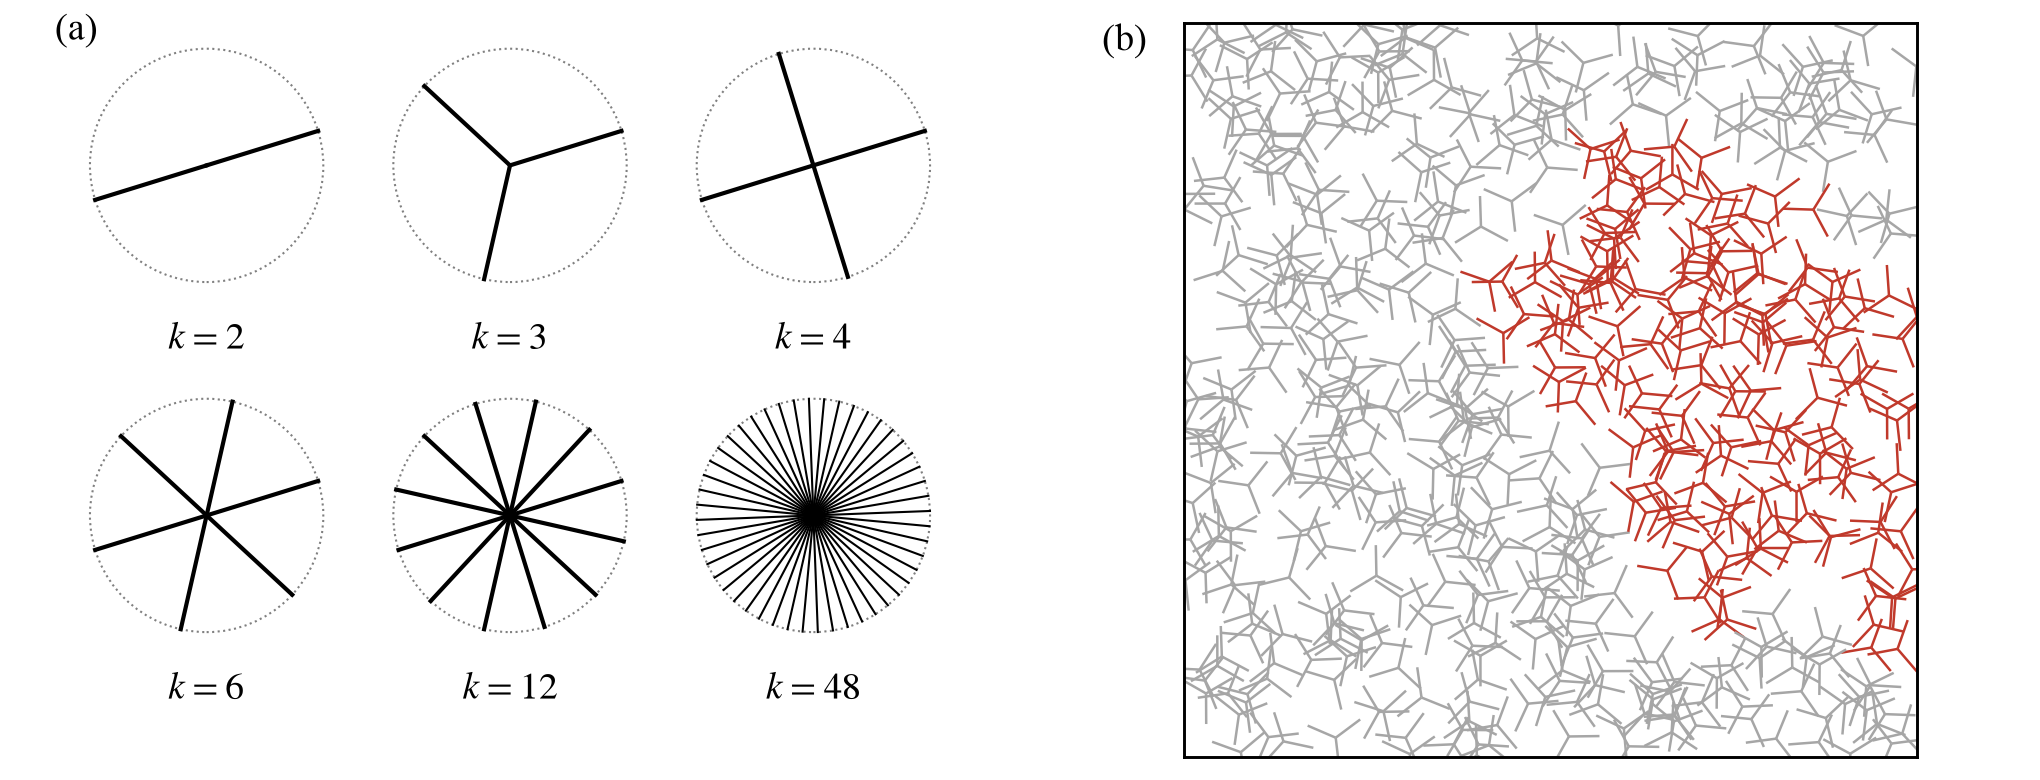
\includegraphics[width=0.92\textwidth]{fig1_stars.png}
\caption{(a) $k$ 本腕の星（点線は半径 $a$ の円）。(b) $k=3$ の星を臨界密度付近で配置した例（$12\times12$ の領域）。赤は最大クラスター。}
\label{fig:stars}
\end{figure*}

\section{モデルと数値計算の方法}
一辺 $L$ の周期境界の正方形に，星の中心を一様に，向きを $[0,2\pi/k)$ で一様に置く。
いずれかの腕どうしが交われば，二つの星は接続しているとみなす。
参照値は，棒が $n_ca^2=5.6372858/4=1.4093215$，円板が $\nd a^2=1.12808737/\pi=0.3590819$ である\cite{Mertens2012}。

Newman--Ziff 法\cite{NewmanZiff2001}とその連続体版\cite{Mertens2012}に従い，星を一つずつ加えながら union--find でクラスターを管理した。
周期境界を一周するクラスター（巻きつき）が初めて現れた時点の数 $N_h$（横方向）と $N_e$（どちらかの方向）を記録した。
巻きつき確率 $R(n)=\langle\Pr[\mathrm{Pois}(nL^2)\ge N]\rangle$ が厳密値 $R_h^*=0.521058$，$R_e^*=0.690474$\cite{Pinson1994}に等しくなる $n$ を $n_c(L)$ とした。
$k\le48$ では $L=16$〜$128$ の結果を $L^{-2}$ で外挿した。
$k\ge64$ では $L=64$ で $2\times10^5$ 回，$L=128$ で $4\times10^4$ 回の試行を行い，両者は誤差の範囲で一致した。
$k$ が大きい場合の接触判定には，腕を相手の円板で切り取り，その部分を見込む角度の範囲に相手の腕が入るかを調べる $O(k)$ の方法を用いた。
この方法は総当たりの判定と $1.3\times10^6$ 通りの配置で一致した。

\section{二つの星の接触条件と格子表現}
$a=1$，$h=2\pi/k$，中心間距離を $r=2(1-\varepsilon)$ とし，
$D(k)=4\pi-\Aex=8\pi\int_0^1(1-\varepsilon)[1-P_k(\varepsilon)]\,d\varepsilon$ とおく。

\begin{lemma}
A の腕が線分 AB となす角を $\alpha$，B の腕が BA となす角を $\beta$ とする（同じ側を正にとる）。
$r>1$ のとき，二本の腕が交わる必要十分条件は，$\alpha,\beta$ が同符号で
\begin{equation}
r\sin|\beta|\le\sin(|\alpha|+|\beta|),\quad r\sin|\alpha|\le\sin(|\alpha|+|\beta|)\label{eq:contact}
\end{equation}
を満たすことである（正弦定理による）。
\end{lemma}
$S_r$ を式\eqref{eq:contact}を満たす $\alpha,\beta>0$ の集合とし，$T_r=S_r\cup(-S_r)$ とおく。
$r$ が小さいほど条件は弱くなるので，$r<r'$ なら $S_r\supseteq S_{r'}$ である。

\begin{lemma}
腕の角度の組は，一様な乱数ずれ $s$ を用いて $s+h\mathbb Z^2$ と書ける。よって
\begin{equation}
P_k(r)=\bigl|T_r\bmod h\mathbb Z^2\bigr|/h^2 .\label{eq:lattice}
\end{equation}
\end{lemma}

$u=(\alpha+\beta)/2$，$\delta=\alpha-\beta$ とおくと，
\begin{equation}
S_r=\{|\delta|\le g_\varepsilon(u)\},\quad g_\varepsilon(u)=2\Bigl[\arcsin\frac{\sin2u}{2(1-\varepsilon)}-u\Bigr]\label{eq:g}
\end{equation}
と書ける。$u=\sqrt\varepsilon\,v$ と置いて展開すると，$\delta$ 方向の半幅は次のようになる。
\begin{equation}
\delta_{\max}(\varepsilon)=c\,\varepsilon^{3/2}\Bigl(1+\frac54\varepsilon+O(\varepsilon^2)\Bigr),\qquad c=\frac{4\sqrt6}{9}\label{eq:dmax}
\end{equation}

\begin{proposition}
$\eta=\frac{h^2}{8}\sup|g''_\varepsilon|$ とおくと，
\begin{equation}
\min\Bigl\{1,\frac{2(\delta_{\max}-\eta)}{h}\Bigr\}\le P_k\le\min\Bigl\{1,\frac{2\delta_{\max}}{h}\Bigr\}.\label{eq:bounds}
\end{equation}
$2(\delta_{\max}-\eta)\ge h$ ならば，向きによらず必ず接触する。
\end{proposition}

\begin{figure*}[tb]
\centering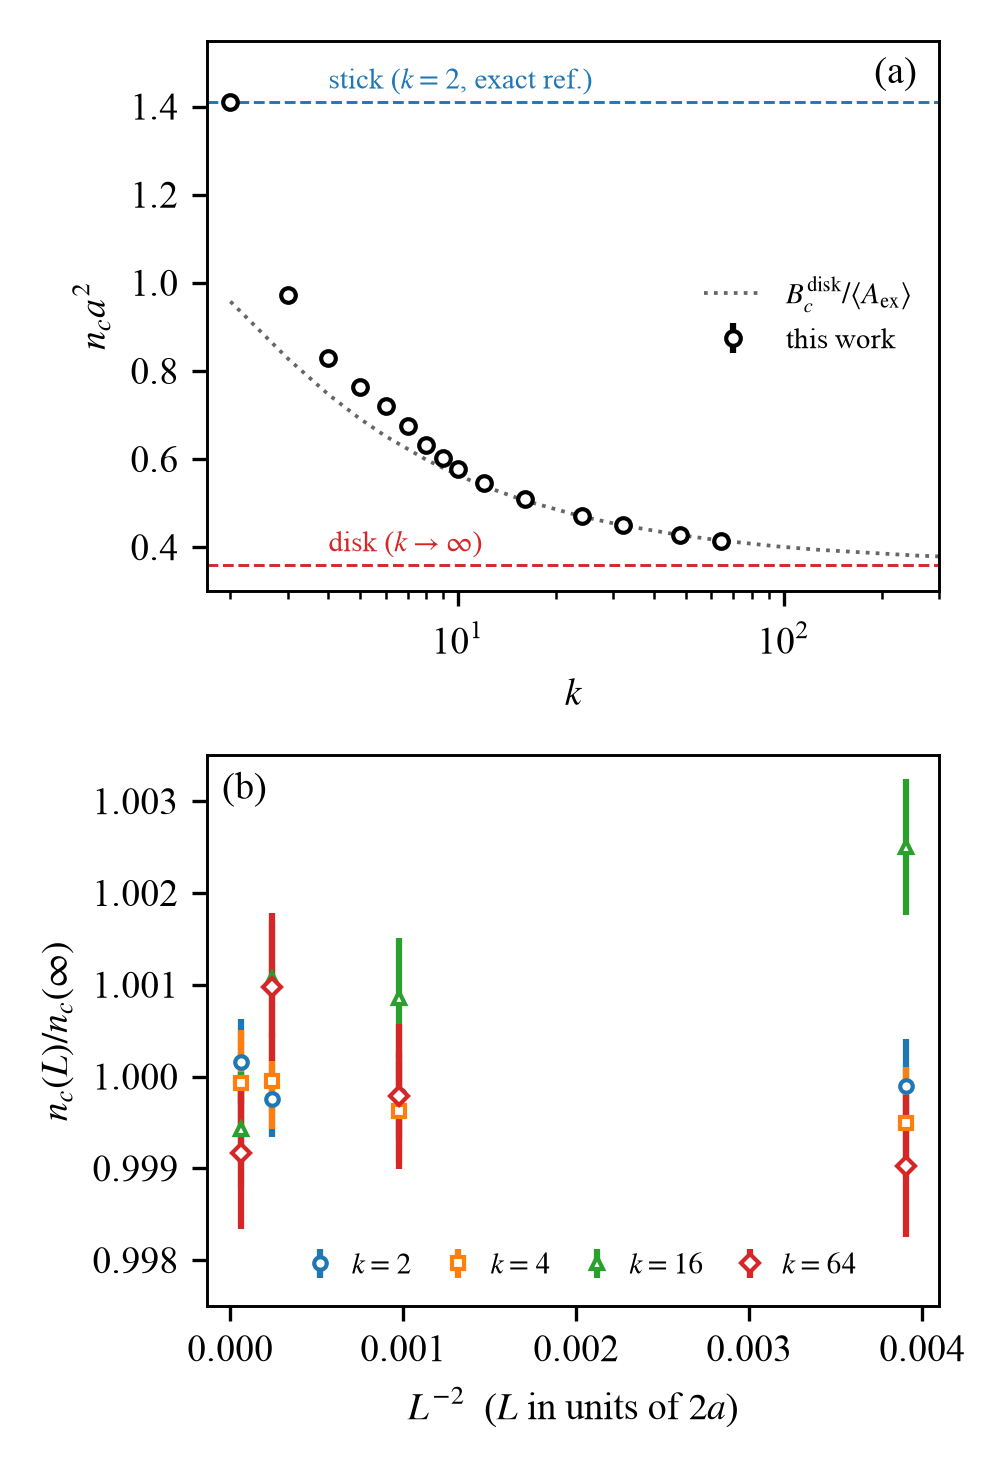
\includegraphics[width=0.92\textwidth]{fig2_threshold.png}
\caption{(a) $n_ca^2$ の $k$ 依存性。(b) 有限サイズの推定値を外挿値で割ったもの。}
\label{fig:thr}
\end{figure*}
\begin{table}[!b]
\caption{臨界数密度，平均排除面積，臨界平均接触数。括弧内は最終桁の誤差（$1\sigma$）。}
\label{tab:results}
\centering\small
\begin{tabular}{rlll}
\toprule
$k$ & $n_ca^2$ & $\Aex/a^2$ & $B_c$\\
\midrule
\csname @@input\endcsname table_data.tex
\bottomrule
\end{tabular}
\end{table}

\begin{figure*}[tb]
\centering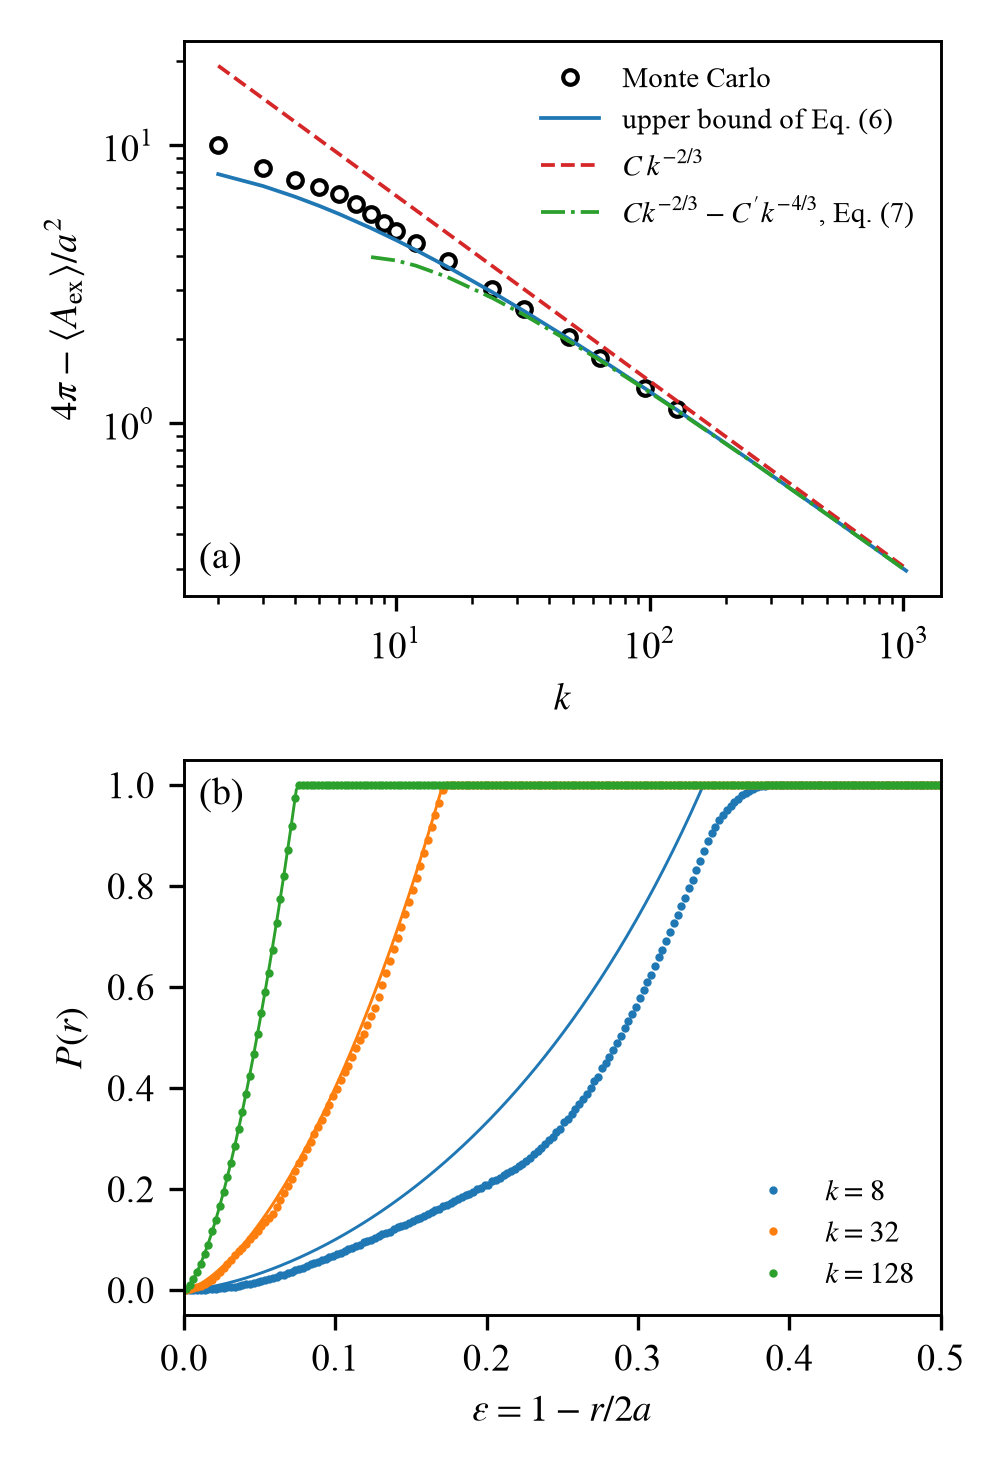
\includegraphics[width=0.92\textwidth]{fig3_excluded.png}
\caption{(a) 排除面積の不足。丸：モンテカルロ，実線：式\eqref{eq:bounds}の上界，破線：$Ck^{-2/3}$，一点鎖線：式\eqref{eq:thm1}。(b) 接触確率 $P(r)$。}
\label{fig:aex}
\end{figure*}

\section{主定理}
$\varepsilon^*=(\pi/ck)^{2/3}$ とする。
\begin{theorem}[排除面積]
$k\to\infty$ で
\begin{equation}
4\pi-\Aex/a^2=Ck^{-2/3}-C'k^{-4/3}+O(k^{-2})\label{eq:thm1}
\end{equation}
が成り立つ。ここで $C=\frac{18}{5}2^{1/3}\pi^{5/3}\approx30.565$，$C'=\frac{36}{7}2^{-1/3}\pi^{7/3}\approx59.00$ である。
誤差項は $k\ge106$ で $2396/k^2$ 以下である。
\end{theorem}
指数 $2/3$ の理由：接触できる角度の幅は $\varepsilon^{3/2}$ でしか広がらず，それが腕の間隔 $h\propto1/k$ に追いつくのは $\varepsilon^*\propto h^{2/3}$ のときである。

\begin{theorem}[臨界密度のはさみうち]
すべての $k$ で $n_c(k)\ge\nd$ であり，$k\ge106$ では
\begin{equation}
\nd\le n_c(k)\le\frac{\nd}{(1-\varepsilon_1)^2},\qquad \varepsilon_1\le1.1\varepsilon^*\label{eq:thm2}
\end{equation}
が成り立つ。
\end{theorem}
\begin{proof}
星は半径 $a$ の円板に含まれるので，星グラフは接続距離 $2a$ の円板グラフの部分グラフである。
逆に，中心間距離が $2a(1-\varepsilon_1)$ 以下の星は必ず接触するので，星グラフは接続距離 $2a(1-\varepsilon_1)$ の円板グラフを含む。
後者の臨界密度は，長さのスケーリングから $\nd/(1-\varepsilon_1)^2$ である。
\end{proof}


\begin{conjecture}\label{conj}
$(n_c-\nd)a^2=\dfrac{\eta_cC}{4\pi^2}k^{-2/3}+o(k^{-2/3})$，$\eta_cC/4\pi^2\approx0.873$。
同値な言い方として，$B_c=B_c^{\rm disk}+o(k^{-2/3})$。
\end{conjecture}
\noindent\textit{予想の根拠．}
星グラフと円板グラフが違うのは，縁の細い帯で辺が欠けることだけである。
臨界密度が接続関数について微分可能で，その感度が $r=2a$ で連続だと仮定すると，変化量は $K(2a)D(k)$ となる。
半径を縮める相似変換から $K(2a)=\nd/4\pi a^2$ と決まり，予想が従う。
ただし，この微分可能性と連続性は連続体パーコレーションでは証明されていない。

\begin{figure*}[tb]
\centering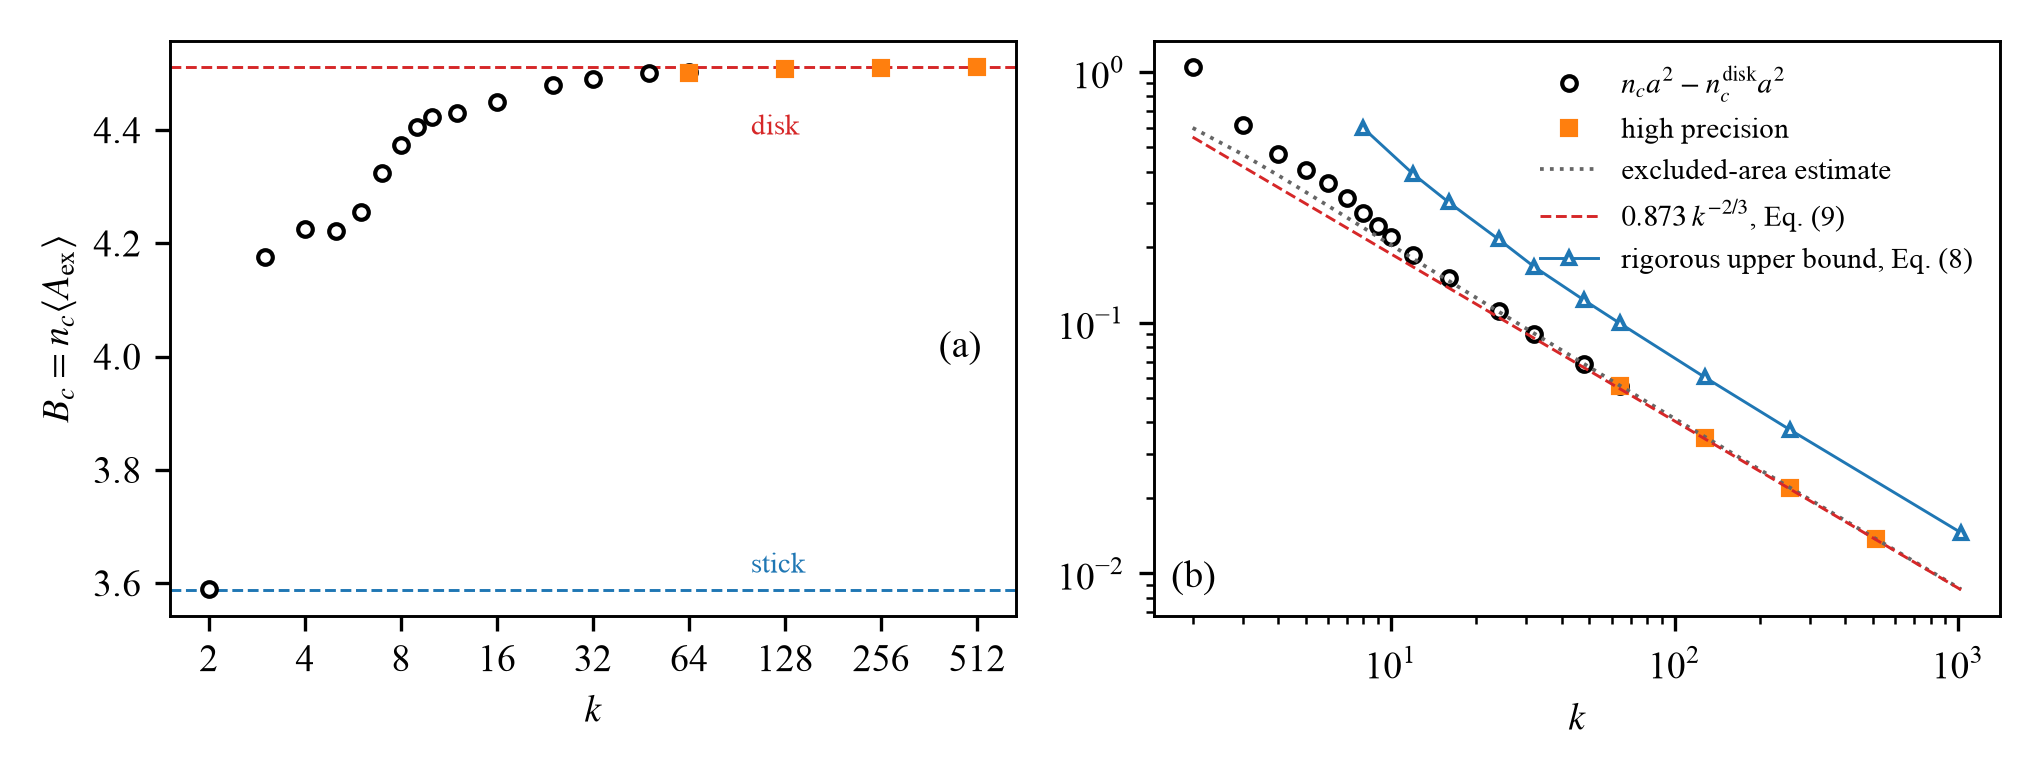
\includegraphics[width=0.92\textwidth]{fig4_Bc.png}
\caption{(a) $B_c=n_c\Aex$。(b) $(n_c-\nd)a^2$。三角は定理2の厳密な上界，破線は予想\ref{conj}。四角は高精度計算。}
\label{fig:bc}
\end{figure*}
\begin{figure*}[tb]
\centering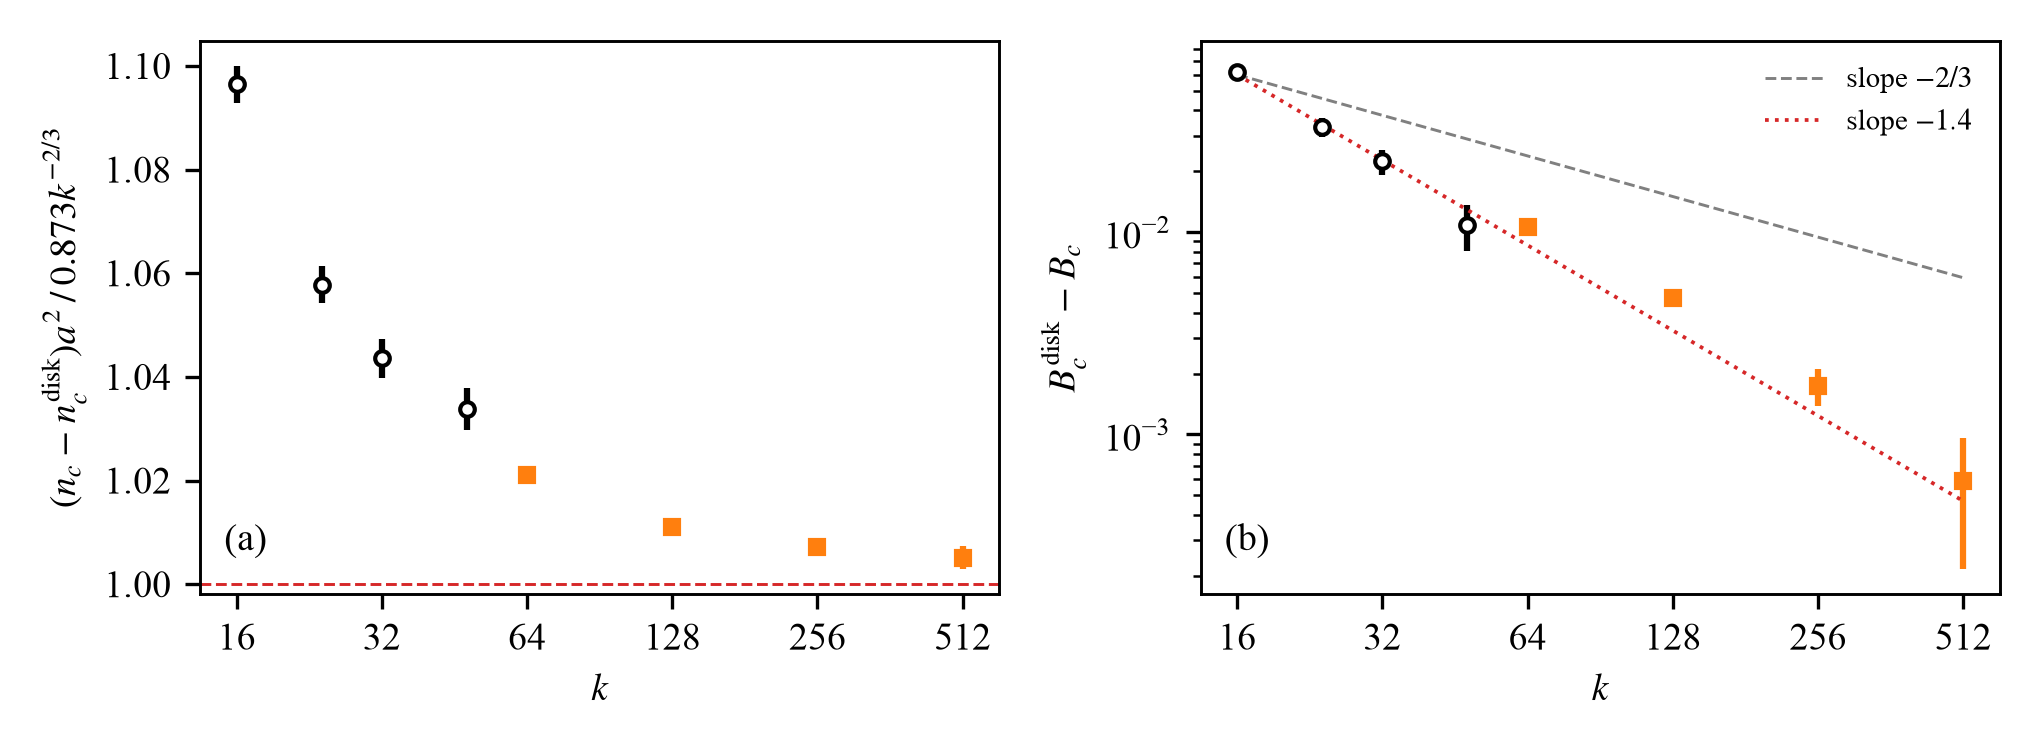
\includegraphics[width=0.92\textwidth]{fig5_conjecture.png}
\caption{予想\ref{conj}の検定。(a) 臨界密度の変化を $0.873k^{-2/3}$ で割ったもの。(b) $B_c^{\rm disk}-B_c$。}
\label{fig:conj}
\end{figure*}

\section{数値結果}
臨界数密度などを表\ref{tab:results}と図\ref{fig:thr}に示す。
$k=2$ では $1.4095(6)$ を得て，厳密値と一致した。
すべての値は定理2の範囲に入っている（例：$k=64$ で $0.3591\le0.4148\le0.4587$）。



排除面積の不足（図\ref{fig:aex}）では，定理1の2項の式が $k=512, 1024$ で4桁一致した。
主要項だけでは $k=1024$ でも $2\%$ ずれる。
$k\ge128$ の高精度モンテカルロ値も，証明した誤差の範囲内にある。


$B_c$ は $k=2$ の $3.590$ から $k=3$ で $4.176$ に跳び，円板の値 $4.5123$ に近づく（図\ref{fig:bc}）。
$k=4$〜$6$ ではほぼ横ばいだった。
$k=7, 9$ の追加計算から，偶奇性による振動ではないことが分かった。
予想\ref{conj}の検定（図\ref{fig:conj}）では，比 $(n_c-\nd)a^2/(0.873k^{-2/3})$ が $k=64,128,256,512$ で $1.021$，$1.011$，$1.007$，$1.005$ と 1 に近づいた。
また $B_c^{\rm disk}-B_c$ は $0.0106$，$0.0047$，$0.0017$，$0.0006$ とおよそ $k^{-1.4}$ で減少し，予想が要求する $o(k^{-2/3})$ と整合する。


\section{考察}
正則な星の接触確率は格子の被覆問題に厳密に帰着でき，これにより $k^{-2/3}$ という遅い収束を証明できた。
定理2は，円板の臨界値を知らずに収束の速さを抑える。
係数 0.873 は予想にとどまるが，数値は $0.5\%$ の精度でこれを支持する。
定理1の証明の一部は計算機援用であり，検証プログラムの正しさに依存している。
実際の分岐粒子では腕の太さやばらつきがあり，$k^{-2/3}$ 則が成り立つ範囲を変えうる。

\section*{データとコード}
コード・生データ・証明ノート・計算機援用の検証は \url{\RepoURL} で公開している（コード：MIT，データと本文：CC BY 4.0）。

\section*{著者貢献と生成AIの利用}
\ContribJa\
本研究では，解析・コード作成・原稿の起草を含め，生成AI（Anthropic 社 Claude）を広く利用した。コードとデータはすべて公開している。内容の責任は著者が負う。

\begin{thebibliography}{99}\small
\bibitem{Stauffer1994} D. Stauffer and A. Aharony, \textit{Introduction to Percolation Theory}, 2nd ed. (Taylor \& Francis, 1994).
\bibitem{Balberg1984} I. Balberg \textit{et al.}, Phys. Rev. B \textbf{30}, 3933 (1984).
\bibitem{Mertens2012} S. Mertens and C. Moore, Phys. Rev. E \textbf{86}, 061109 (2012).
\bibitem{Baker2002} D. R. Baker \textit{et al.}, Phys. Rev. E \textbf{66}, 046136 (2002).
\bibitem{Pike1974} G. E. Pike and C. H. Seager, Phys. Rev. B \textbf{10}, 1421 (1974).
\bibitem{Li2013} J. Li and M. \"Ostling, Phys. Rev. E \textbf{88}, 012101 (2013).
\bibitem{Manna2003} L. Manna \textit{et al.}, Nat. Mater. \textbf{2}, 382 (2003).
\bibitem{Geigenfeind2019} T. Geigenfeind and D. de las Heras, J. Chem. Phys. \textbf{150}, 184906 (2019).
\bibitem{RoyTanemura2002} R. Roy and H. Tanemura, Adv. Appl. Probab. \textbf{34}, 48 (2002).
\bibitem{NewmanZiff2001} M. E. J. Newman and R. M. Ziff, Phys. Rev. E \textbf{64}, 016706 (2001).
\bibitem{Pinson1994} H. T. Pinson, J. Stat. Phys. \textbf{75}, 1167 (1994).
\end{thebibliography}

\end{document}
